% !TeX program = xelatex*2
% !TeX root = ../elegantnote.tex
\section{数值逼近}
\subsection{插值法}
\begin{definition}[插值函数]
    已知函数$y = f(x)$在互异节点$\left\{ x_i \right\}_{i = 0}^{n}\subset \left[ a,b \right]$处的函数值$\left\{ y_i = f(x_i) \right\}_{i = 0}^{n}$,若存在简单函数$p(x)$,使得
    \begin{equation}\label{eq:chazhi}
        p(x_i) = y_i,\ (i = 0,1,\dots,n)
    \end{equation}
    成立,则称$p(x)$是$f(x)$关于节点$\left\{ x_i \right\}_{i = 0}^{n}$的一个插值函数。
    $\left\{ x_i \right\}_{i = 0}^{n}$——插值节点,$\left[ a,b \right]$——插值区间,$f(x)$——被插值函数。
\end{definition}
\begin{note}
    用$p(z)$的值作为$f(z)$的近似值,当元在节点形成的区间上时,称该方法为内插法﹔当元不在节点形成的区间上但在插值区间上,则称该方法为外插法。
\end{note}
\begin{note}
    当插值函数$p(z)$为多项式时,称 $p(x)$是$f(x)$的一个插值多项式。插值余项$R(x)\overset{\text{def}}{=}f(x)-p(x)$,插值余项又称为截断误差。
\end{note}
\begin{theorem}[插值多项式的存在惟一性定理]
    满足插值条件(\ref{eq:chazhi})的不超过$n$次的插值多项式$p(x)$是存在唯一的。
\end{theorem}
\begin{corollary}
    若$f(\alpha)$是不超过$n$次的多项式,则它的关于$n+1$个互异节点$\left\{ x_i \right\}_{i = 0}^{n}$的不超过$n$次的插值多项式$p(x)$与被插值函数$f(x)$恒等,即有
    \[
        p(x)\equiv f(x)
    \]
\end{corollary}
\begin{note}
    误差的估计:
    \begin{itemize}
        \item 若被插值函数$f(x)\in \boldsymbol{C}^{n+1}\left[ a,b \right]$,则有插值误差估计式
        \[
            \left| R_{n}(x) \right|\leqslant \dfrac{M_{n+1}}{(n+1)!}\left| \omega_{n+1}(x) \right|
        \]
        \item 若仅需估计某一点$\bar{x}^*$处的插值误差,则利用
        \[
            \left| R(\bar{x}) \right|\leqslant \dfrac{M_{n+1}}{(n+1)!}\left| \omega_{n+1}(\bar{x}) \right|,\,\bar{x} \in \left[ a,b \right]
        \]
        \item 若要估计在整个插值区间上的误差,用
        \[
            \left| R(\bar{x}) \right|\leqslant \dfrac{M_{n+1}}{(n+1)!}\left| \omega_{n+1}(x) \right|,\,\forall x \in \left[ a,b \right]
        \]
        其中,$M_{n+1}$和$\max\limits_{x\in [a,b]} |\omega_{n+1}(x)|$用微积分中求极值的方法进行。
    \end{itemize}
\end{note}
\subsection{Lagrange插值}
设$p(x)$是形如$p(x) = a_0+a_1x+a_2x^2+\cdots+a_nx^n$,根据$n+1$个互异节点$\left\{ x_i \right\}_{i = 0}^{n}$,得到
\[
    \begin{cases}a_0+a_1x_0+\cdots+a_nx_0^n=y_0,\\a_0+a_1x_1+\cdots+a_nx_1^n=y_1,\\\vdots\\a_0+a_1x_n+\cdots+a_nx_n^n=y_n.\end{cases}
\]
因为
\[
    V_n(x_0,x_1,\cdots,x_n)=\left.\left|\begin{array}{ccccc}1&x_0&x_0^2&\cdots&x_0^n\\1&x_1&x_1^2&\cdots&x_1^n\\\vdots&\vdots&\vdots&&\vdots\\1&x_n&x_n^2&\cdots&x_n^n\end{array}\right.\right|\neq 0
\]
所以方程存在唯一一组解$a_0,a_1,\cdots,a_n$,故而拉格朗日插值多项式也存在且唯一。
\[
    p_n(x) = L_n(x) = \sum\limits_{i = 0}^{n}f(x_i)l_i(x)
\]
拉格朗日插值多项式需要满足$p_{n}(x_i) = f(x_i)$,故而$n$次多项式$l_i(x)$需要满足
\[
    l_i(x_j) = \left\{
        \begin{array}{ll}
            1, & j = i\\
            0, & j\neq i
        \end{array}
    \right.
\]
可以将拉格朗日插值基函数$\left\{ l_i(x) \right\}_{i = 0}^{n}$的定义如下:
\[
    l_{i}(x) = \prod\limits_{\substack{j = 0\\ j\neq i}}\dfrac{x-x_j}{x_i-x_j} = \dfrac{\omega_{n+1}(x)}{(x-x_i)\omega_{n+1}'(x_i)}
\]
其中
\[
    \begin{array}{l}

        \omega_{n+1}(x) = (x-x_0)(x-x_1)\cdots(x-x_n)\\
        \omega'_{n+1}(x_k) = (x_k-x_0)\cdots(x_k-x_{k-1})(x_k-x_{k+1})(x_k-x_n)\\
    \end{array}
\]
\begin{theorem}[插值余项定理]
    设$f^{n}(x)$在$\left[ a,b \right]$上连续,$f^{n+1}(x)$在$\left( a,b \right)$上存在,节点$a\leqslant x_0<x_1<\cdots<x_n\leqslant b$,$L_{n}(x)$是满足条件$p_{n}(x_i) = f(x_i)$的多项式,则对任何$x\in\left[ a,b \right]$,插值余项
    \[
        R_n(x) = f(x)-L_n(x) = \dfrac{f^{(n+1)}(\xi)}{(n+1)!}\omega_{n+1}(x)
    \]
    这里,$\xi\in(a,b)$且依赖于$x$。
\end{theorem}
\begin{proof}
    由给定条件知,$R_n(x)$在$\left\{ x_i \right\}_{i = 0}^{n}$上为0,即
    \[
        R_n(x_i) = 0
    \]
    于是
    \[
        R_n(x) = K(x)\omega_{n+1}(x)
    \]
    其中$K(x)$是与$x$有关的待定系数。
    现在把$x$看成$\left[ a,b \right]$上的一个固定点,做函数
    \[
        \phi(t) = f(t)-L_n(t)-K(x)\omega_{n+1}(t)
    \]
    容易知道$\phi(t)$在点$x,x_0,\cdots,x_n$这$n+2$个点上满足$\phi(t) = 0$,反复利用Rolle定理,知道
    \[
        \phi^{(n+1)}(\xi) = f^{(n+1)}(\xi)-(n+1)!K(x) = 0
    \]
    于是
    \[
        K(x) = \dfrac{f^{(n+1)(\xi)}}{(n+1)!}
    \]
    证毕!
\end{proof}
\begin{remark}
    $\xi$在$(a,b)$内的具体位置通常不可能给出,如果可以求出$\max\limits_{a\leqslant x\leqslant b}|f^{(n+1)}(x)| = M_{n+1}$,那么插值多项式$L_n(x)$逼近$f(x)$的截断误差是
    \[
        |R_n(x)|\leqslant \dfrac{M_{n+1}}{(n+1)!}|\omega_{n+1}(x)|
    \]
\end{remark}
\begin{corollary}
    若$f(x)$是不超过$n$次的多项式,则它的关于$n+1$个互异节点$\left\{ x_i \right\}_{i = 0}^{n}$$n$次的拉格朗日插值多项式$L_{n}(x)$有
    \[
        R_{n}(x) = f(x)-L_{n}(x) = 0
    \]
    即
    \[
        f(x) = L_{n}(x) = \sum\limits_{i = 0}^{n}f(x_i)l_{i}(x)
    \]
\end{corollary}
\begin{example}
    证明$\sum\limits_{i = 0}^{5}\left( x-x_i \right)^2l_{i}(x) = 0$,其中$l_{i}(x)$是关于$\left\{ x_0,x_1,\cdots, x_5 \right\}$的插值基函数。\Stars{5}
    \begin{proof}
        \[
            \begin{array}{ll}
                \sum\limits_{i = 0}^{5}\left( x-x_i \right)^2l_{i}(x) & = x^2\sum\limits_{i = 0}^{5}1\cdot l_{i}(x)-2x\sum\limits_{i = 0}^{5}x_i\cdot l_{i}(x)+\sum\limits_{i = 0}^{5}x_{i}^2\cdot l_{i}(x)\\
                &=x^2-2x\cdot x+x^2 = 0
            \end{array}
        \]
        证毕!
    \end{proof}    
\end{example}
\begin{example}
    对一条直线采样10个点进行Lagrange插值,所得插值多项式是\sol{1}次的。
\end{example}
\begin{note}
    Aitken逐次线性插值法:

    用Lagrange插值多项式$L_{n}(x)$计算函数近似值时,如需增加插值节点,那么原来算出来的数据均不能利用,必须重新计算。为克服这个缺点通常可用逐次线性插值方法得到高次插值。

    两个$k$次插值多项式可通过线性插值得到$k+1$次插值多项式
    \begin{equation}\label{eq:Aitken}
        I_{0,1,\cdots,k,l}(x) = I_{0,1,\cdots,k}(x)+\dfrac{I_{0,1,\cdots,k-1,l}(x)-I_{0,1,\cdots,k}(x)}{x_l-x_k}\left( x-x_k \right)
    \end{equation}
    这是关于节点$\left\{ x_0,\cdots,x_{k},x_{l} \right\}$的插值多项式。显然
    \begin{itemize}
        \item 对于$i = 0,1,\cdots,k-1$
        \[
            I_{0,1,\cdots,k,l}(x_i) = I_{0,1,\cdots,k}(x_i) = f(x_i)
        \]
        \item 对于$x_k$
        \[
            I_{0,1,\cdots,k,l}(x_k) = I_{0,1,\cdots,k}(x_k) = f(x_k)
        \]
        \item 对于$x_l$
        \[
            I_{0,1,\cdots,k,l}(x_l) = I_{0,1,\cdots,k}(x_l)+\dfrac{f(x_l)-I_{0,1,\cdots,k}(x_l)}{x_l-x_k}(x_l-x_k) = f(x_l)
        \]
    \end{itemize}
    这证明了(\ref{eq:Aitken})满足插值条件。

    当$k = 0$时为线性插值,当$k = 1$时插值节点为$x_0,x_1,x_l$,插值多项式为
    \[
        I_{0,1,l}(x) = I_{0,1}(x)+\dfrac{I_{0,l}(x)-I_{0,1}(x)}{x_l-x_1}(x-x_1)
    \]
    % Table generated by Excel2LaTeX from sheet 'Aitken逐次线性插值'
    \begin{table}[htbp]
        \centering
        \begin{tabular}{|c|c|c|c|c|c|c|}
            \hline
            $x_0$ & $f(x_0)$ &     &     &     &     & $x-x_0$ \bigstrut\\
            \hline
            $x_1$ & $f(x_1)$ & $I_{0,1}$ &     &     &     & $x-x_1$ \bigstrut\\
            \hline
            $x_2$ & $f(x_2)$ & $I_{0,2}$ & $I_{0,1,2}$ &     &     & $x-x_2$ \bigstrut\\
            \hline
            $x_3$ & $f(x_3)$ & $I_{0,3}$ & $I_{0,1,3}$ & $I_{0,1,2,3}$ &     & $x-x_3$ \bigstrut\\
            \hline
            $x_4$ & $f(x_4)$ & $I_{0,4}$ & $I_{0,1,4}$ & $I_{0,1,2,4}$ & $I_{0,1,2,3,4}$ & $x-x_4$ \bigstrut\\
            \hline
        \end{tabular}%
  \end{table}%
\end{note}
\subsection{Newton插值}
\[
    p_{n}(x) = N_{n}(x) = \sum\limits_{i = 0}^{n}f\left[ x_0,x_1,\cdots,x_i \right]\omega_{i}(x)
\]
其中零阶插商
\[
    f\left[ x_0 \right] = f(x_0),\,\omega_0(x)\equiv 1,\,\omega_{i}(x) = \prod\limits_{k = 0}^{i-1}(x-x_k)
\]
\begin{definition}[差商]
    称$f\left[ x_0,x_k \right]=\dfrac{f(x_k)-f(x_0)}{x_k-x_0}$为函数$f(x)$关于$x_0,x_k$的一阶差商,称
    \[
        f\left[ x_0,x_l,x_k \right] = \dfrac{f\left[ x_0,x_k \right]-f\left[ x_0,x_l \right]}{x_k-x_l}
    \]
    为$f(x)$关于$x_0,x_k,x_l$的二阶差商。一般的称
    \[
        f[x_0,x_1,\cdots,x_m]=\frac{f[x_0,x_1,\cdots,x_{k-2},x_m]-f[x_0,x_1,\cdots,x_{k-2},
        x_{k-1}]}{x_m-x_{k-1}}
    \]
    为$f(x)$的$k$阶差商。
\end{definition}
\begin{note}
    插值误差:把$x$当作$[a,b]$一点,可得
    \[
        \begin{array}{c}
            f(x) = f(x_0)+f\left[ x,x_0 \right](x-x_0)\\
            f(x) = f(x_0)+f\left[ x_0,x_1 \right](x-x_0)+f\left[ x,x_0,x_1 \right](x-x_0)(x-x_1)\\
            \cdots\\
            \begin{array}{ll}
                f(x) &= f(x_0)+f\left[ x_0,x_1 \right](x-x_0)\\
                &+f\left[x_0,x_1,x_2 \right](x-x_0)(x-x_1)+\cdots\\
                &+f\left[ x_0,\cdots,x_n \right](x-x_0)\cdots(x-x_{n-1})\\
                &+f\left[ x,x_0,\cdots,x_n \right]\prod\limits_{i = 0}^{n}(x-x_i)\to\textcolor{red}{\text{插值误差\ or\ }\text{余项}R_{n}(x)}
            \end{array}
        \end{array}  
    \]
    由上,得
    \[
        \begin{array}{c}
            f(x) = N_n(x)+f\left[ x,x_0,\cdots,x_n \right]\prod\limits_{i = 0}^{n}(x-x_i)\\
            \text{和拉格朗日插值对比}\\
            f(x) = L_{n}(x)+\dfrac{f^{(n+1)}(\xi)}{(n+1)!}\omega_{n+1}(x)
        \end{array}
    \]
\end{note}



\begin{note}
    差商有如下性质:
    \begin{enumerate}
        \item $k$阶差商可表示为函数值$f(x_{0}),\cdots,f(x_k)$的线性组合,即
        \[
            f[x_0,x_1,\cdots,x_k]=\sum\limits_{j=0}^k\frac{f(x_j)}{(x_j-x_0)\cdotp\cdotp\cdotp(x_j-x_{j+1})(x_j-x_{j+1})\cdotp\cdotp\cdotp(x_j-x_k)}.
        \]
        这个性质也表明差商与节点的排列顺序无关(插值的对称性)。
        \item 差商与导数的关系
        \begin{equation}\label{eq:MinusQution}
            f[x_0,x_1,\cdots,x_n]=\frac{f^{(n)}(\xi)}{n!},\quad\xi\in[a,b].
        \end{equation}
        \begin{proof}
            \[
                f(x) = N_{n-1}(x)+f\left[ x,x_0,\cdots,x_{n-1} \right]\omega_{n}(x)
            \]
            记$R(x) = f(x)-N_{n-1}(x) = f\left[ x,x_0,\cdots,x_{n-1} \right]\omega_{n}(x)$,固定$x$,令
            \[
                g(t) = f(t)-N_{n-1}(x)-f\left[ x,x_0,\cdots,x_{n-1} \right]\omega_{n}(t)
            \]
            对于$\left\{ x,x_0,\cdots,x_{n-1} \right\}$有
            \[
                g(x) = g(x_0) = \cdots = g(x_{n-1}) = 0    
            \]
            反复利用Rolle定理,得到
            \[
                g^{(n)}(\xi) = f^{(n)}(\xi)-f\left[ x,x_0,\cdots,x_{n-1} \right]n! = 0
            \]
            即(这一步将$x_n$带入$x$,并利用插值的对称性)
            \[
                f[x_0,x_1,\cdots,x_n]=\frac{f^{(n)}(\xi)}{n!},\quad\xi\in[a,b].
            \]
            证毕!
        \end{proof}
    \end{enumerate}
\end{note}
\begin{figure}[htbp]
    \centering
    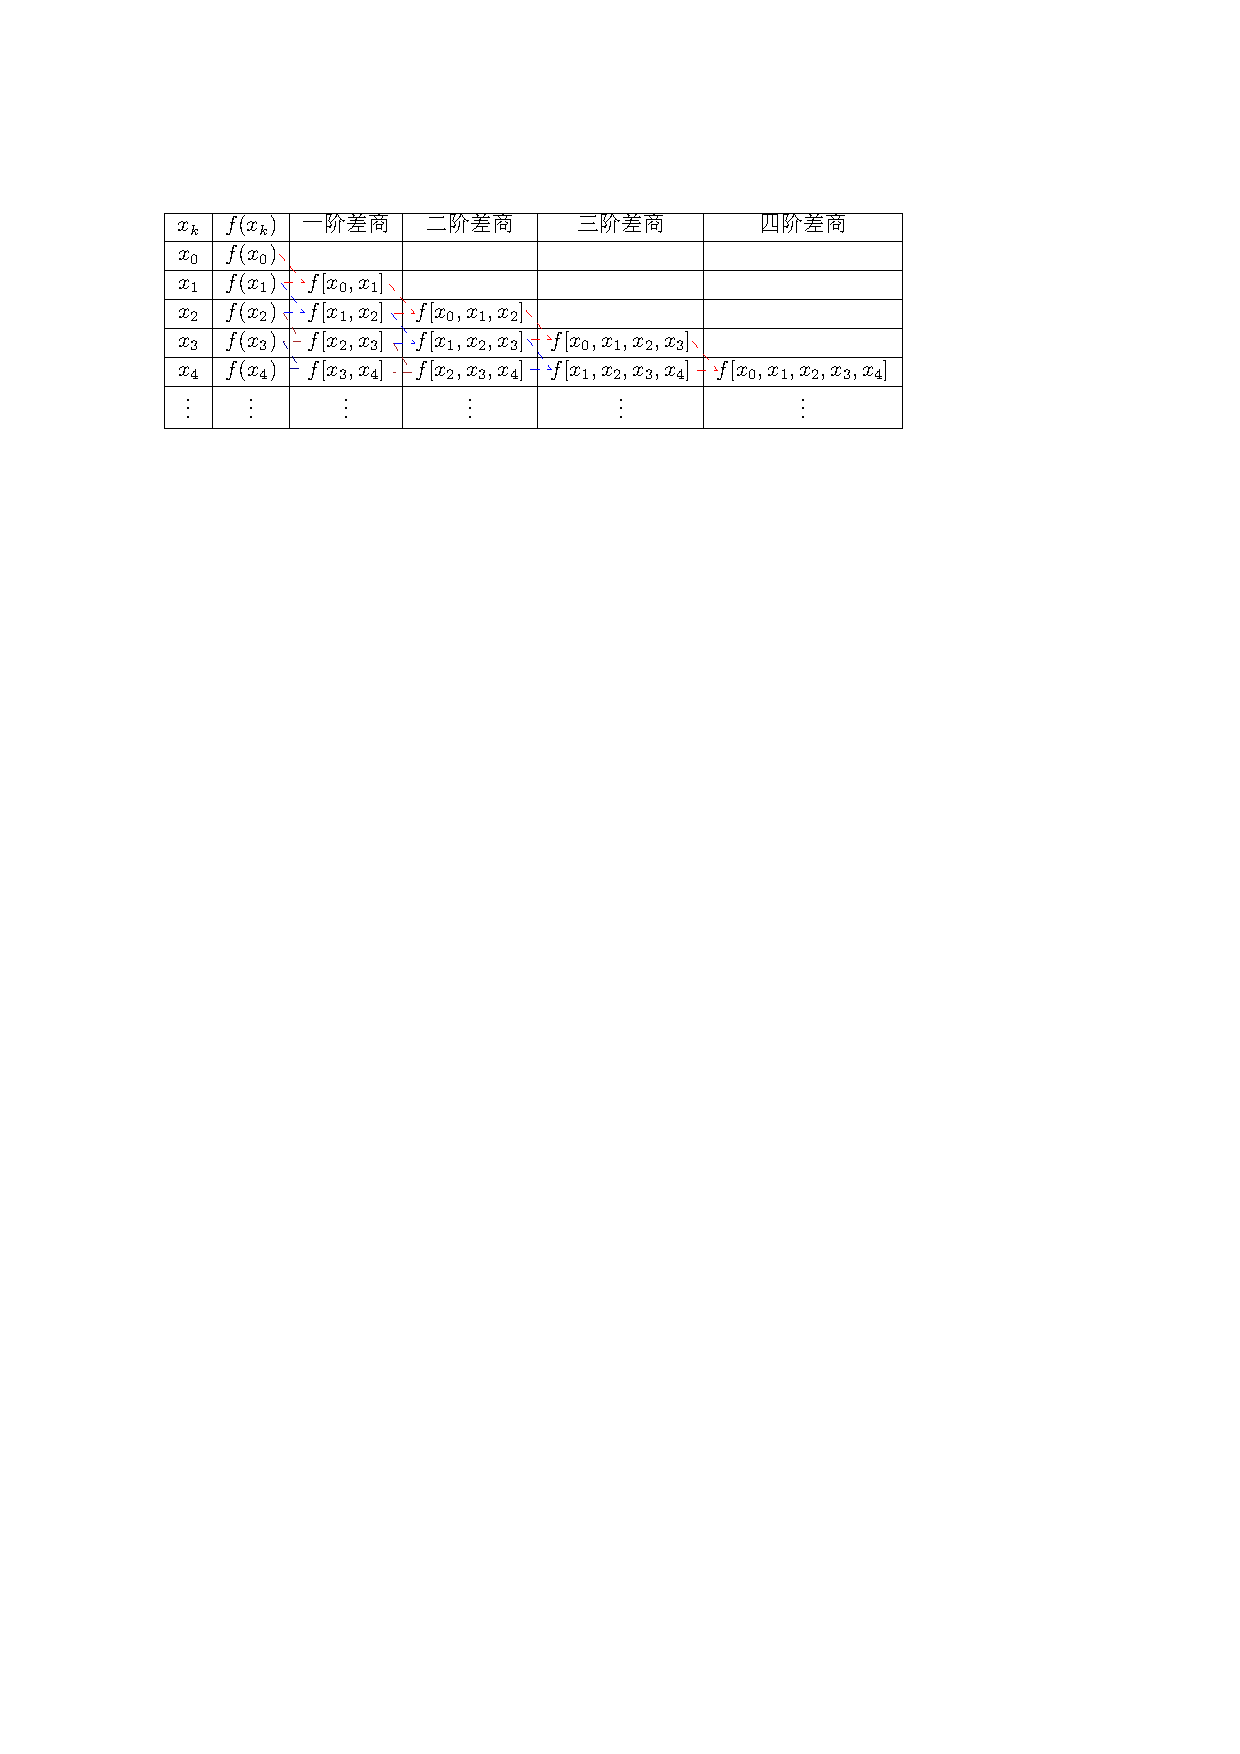
\includegraphics{image/Newton插值表.pdf}
\end{figure}
\subsubsection{差分与等距节点插值公式}
设等式$y = f(x)$在等距节点$x_k = x_0+kh\,(k = 0,1,\cdots,n)$上的值$f_k = f(x_k)$为已知,这里$h$为常数,称为步长。
\begin{definition}[偏差]
    \[
        \begin{array}{c}
            \Delta f_k = f_{k+1}-f_k\\
            \nabla f_k = f_{k}-f_{k-1}\\
            \delta f_k=f(x_k+h/2)-f(x_k-h/2)=f_{k+\frac12}-f_{k-\frac12}
        \end{array}
    \]
    分别为向前差分、向后差分以及中心差分。
\end{definition}
\begin{corollary}[差商与差分的关系\Stars{5}]
    \[
        f\left[ x_k,x_{k+1},\cdots,x_{k+m} \right] = \dfrac{1}{m!}\dfrac{1}{h^m}\Delta^mf_{k},\,(m = 1,2,\cdots,n)
    \]
    \[
        f\left[ x_k,x_{k-1},\cdots,x_{k-m} \right] = \dfrac{1}{m!}\dfrac{1}{h^m}\Delta^mf_{k}
    \]
    同时利用(\ref{eq:MinusQution})可以得到
    \[
        \Delta^nf_{k} = h^nf^{(n)}(\xi),\,\xi\in(x_k,x_{k+n})
    \]
\end{corollary}

\subsection{Hermite插值}
不少实际问题不但要求在节点上函数值相等,而且还要求它的导数值相等,甚至要求高阶导数值也相等.满足这种要求的插值多项式就是Hermite插值多项式.

已知节点$\left\{ x_{j} \right\}_{j = 0}^{n}$,满足
\[
    H(x_j) = y_{j},\,H^{\prime}(x_{j}) = m_{j} = f^{\prime}(x_{j})
\]
可以确定$2n+1$次的多项式
\begin{equation}\label{eq:2n+1Hermite}
    H_{2n+1}(x) = a_0+a_1x+\cdots+a_{2n+1}x^{2n+1}
\end{equation}
插值误差
\[
    R_{n}(x)  =\dfrac{f^{(2n+2)}(\xi)}{(2n+2)!}\omega_{n+1}^2(x)
\]
用基函数表示(\ref{eq:2n+1Hermite})为
\[
    H_{2n+1}(x) = \sum\limits_{i = 0}^{n}\left[ \alpha_{i}(x)f_{i}+\beta_{i}(x)f'_{i} \right]
\]
其中$\alpha_{i}(x)$和$\beta_{i}(x)$均为$2n+1$次多项式,且满足
\begin{equation}\label{eq:constrainHermit}
    \left\{
        \begin{array}{ll}
            \alpha_{i}(x_k) = \delta_{ik}, & \alpha_{i}^{\prime}(x_k) = 0\\
            \beta_{i}(x_k) = 0, & \beta_{i}^{\prime}(x_k) = \delta_{ik}\\
        \end{array}
    \right.
\end{equation}
\begin{note}
    下面的问题就是求满足条件(\ref{eq:constrainHermit})的基函数$\alpha_{i}$和$\beta_{i}(x)$。
    \begin{itemize}
        \item 先求$\alpha_{i}(x)$,可利用Lagrange插值基函数$l_{i}(x)$,令(1.$2n+1$次多项式,2.在$x_j \neq x_i$处为2重零点)
        \[
            \alpha_{i}(x) = [a(x-x_i)+b]l_{i}^2(x)
        \]
        其中$l_{i}(x) = \prod\limits_{j = 0,j\neq i}^{n}\dfrac{x-x_j}{x_i-x_j}$。由$\alpha_{i}(x_i) = 1$,知$b = 1$;由$\alpha_{i}^{\prime}(x_i) = 0$知
        \[
            \begin{array}{l}
                al_{i}^2(\colorbox{cyan!50}{$x_i$})+2[a(\colorbox{cyan!50}{$x_i$}-x_i)+1]l_{i}(\colorbox{cyan!50}{$x_i$})l_{i}^{\prime}(\colorbox{cyan!50}{$x_i$}) = 0\\
                a = -2l_{i}^{\prime}(x_i)\\
                \left( \ln l_{i}(x_i) \right)' = \dfrac{l_{i}^{\prime}(x_i)}{l_{i}(\colorbox{cyan!50}{$x_i$})} = \sum\limits_{\substack{j = 0\\j\neq i}}^{n}\dfrac{1}{(x_i-x_j)}\\
                a = -2\sum\limits_{\substack{j = 0\\j\neq i}}^{n}\dfrac{1}{(x_i-x_j)}\\
            \end{array}
        \]
        故而有
        \[
            \alpha_{i}(x) = \left[1-2(x-x_i)\sum\limits_{\substack{j = 0\\j\neq i}}^{n}\dfrac{1}{(x_i-x_j)}\right]l_{i}^2(x)
        \]
        \item 再求$\beta_{i}(x)$,同理设$\beta_{i}(x) = [a(x-x_i)+b]l_{i}^2(x)$(1.$2n+1$次多项式,2.在$x_j \neq x_i$处为2重零点)。由$\beta_{i}(x_i) = 0$,知$b = 0$;由$\beta_{i}^{\prime}(x_i) = 1$知,
        \[
            \begin{array}{l}
                al_{i}^2(\colorbox{cyan!50}{$x_i$})+2[a(\colorbox{cyan!50}{$x_i$}-x_i)+0]l_{i}(\colorbox{cyan!50}{$x_i$})l_{i}^{\prime}(\colorbox{cyan!50}{$x_i$}) = 1\\
                a = 1
            \end{array}
        \]
        故而有
        \[
            \beta_{i}(x) = (x-x_i)l_{i}^2(x)
        \]
    \end{itemize}
    综上,
    \[
        \begin{array}{l}
            \alpha_{i}(x) = \left[1-2(x-x_i)\sum\limits_{j = 0,j\neq i}^{n}\dfrac{1}{(x_i-x_j)}\right]l_{i}^2(x)\\
            \beta_{i}(x) = (x-x_i)l_{i}^2(x)
        \end{array}
    \]
\end{note}
\begin{example}
    设$f(x) = \ln x$,给定$f(1) = 0,f(2) = 0.693147,f'(1) = 1,f'(2) = 0.5$,用三次Hermite插值多项式$H_3(x)$计算$f(1.5)$的近似值。\Stars{5}{}
    
    请写出$x = 1$处的导数值基函数$\beta_1(x)$和$x = 2$处的函数值基函数$\alpha_2(x)$
    \begin{solution}
        $\beta_{1}(x) = (x-1)\left[ \dfrac{(x-2)}{1-2} \right]^2,\quad \alpha_2(x) = \left[ 1-2(x-2)\dfrac{1}{2-1} \right]\left[ \dfrac{(x-1)}{2-1} \right]^2$
    \end{solution}
\end{example}
\begin{example}
    求一个次数不高于四次的多项式$p(x)$,使它满足$p(0) = p'(0) = 0,\,p(1) = p'(1) = 1,\,p(2) = 1$。\Stars{5}{}
    \begin{solution}
        [解法一]:
        设$p(x) = \left[ \alpha_1(x)p(0)+\alpha_2(x)p(1)+\alpha_3(x)p(2) + \beta_1(x)p'(0)+\beta_2(x)p'(1) \right]$,满足
        % Table generated by Excel2LaTeX from sheet 'Hermit插值'
        \begin{table}[htbp]
            \centering
            \begin{tabular}{|c|c|c|c|c|c|}
            \hline
                & \multicolumn{3}{c|}{函数值} & \multicolumn{2}{c|}{导数值} \bigstrut\\
            \hline
                & 0   & 1   & 2   & 0   & 1 \bigstrut\\
            \hline
            $\alpha_1(x)$ & 1   & 0   & 0   & 0   & 0 \bigstrut\\
            \hline
            $\alpha_2(x)$ & 0   & 1   & 0   & 0   & 0 \bigstrut\\
            \hline
            $\alpha_3(x)$ & 0   & 0   & 1   & 0   & 0 \bigstrut\\
            \hline
            $\beta_1(x)$ & 0   & 0   & 0   & 1   & 0 \bigstrut\\
            \hline
            $\beta_2(x)$ & 0   & 0   & 0   & 0   & 1 \bigstrut\\
            \hline
            \end{tabular}%
        \end{table}%
        可以设
        \[
            \begin{array}{l}
                \alpha_{1}(x) = (ax+b)(x-1)^2(x-2) \\
                \alpha_{2}(x) = (ax+b)x^2(x-2) \\
                \alpha_{3}(x) = bx^2(x-1)^2 \\ 
                \beta_{1}(x) = (ax+b)x(x-1)^2 \\
                \beta_{2}(x) = (ax+b)x^2(x-1)
            \end{array}    
        \]
        上述做法要解多个2元方程,虽然每个方程计算量不大。

        [解法二]:可以看出关于$x = 0$为二重根,设$p(x) = (ax^2+bx+c)x^2$,可以通过求解1个三元方程组

        [解法三]:由给定的条件,可确定次数不超过4的插值多项式
        \[
            p(x) = f(0) + f[0,1](x-0) + f[0,1,2](x-0)(x-1) + (ax+b)(x-0)(x-1)(x-2)
        \]
    \end{solution}
\end{example}

\begin{example}
    求次数不高于三次的多项式$p(x)$,使得$p(x_i) = f(x_i)(i = 0,1,2)$及$p'(x_1) = f'(x_1)$的插值多项式\Stars{4}{}
    
    \begin{solution}
        可以设$p(x)$为
        \[
            \begin{array}{l}
                p(x) = f(x_0) + f[x_0,x_1](x-x_0) + f[x_0,x_1,x_2](x-x_0)(x-x_1) + \\
                A(x-x_0)(x-x_1)(x-x_2)
            \end{array}
        \]
        可以得到
        \[
            A = \dfrac{f'(x_1)-f[x_0,x_1]-f[x_0,x_1,x_2](x_1-x_0)}{(x_1-x_0)(x_1-x_2)}
        \]
    \end{solution}
\end{example}

\subsection{分段低次插值}
\subsubsection{分段线性插值}
设已知节点$a=x_0<x_1<\cdots<x_n=b$上的函数值为$f_0,f_{1}, \cdots , f_{n}, h_{i}= x_{i+ 1}- x_{i}$, $h= \max _{0\leq i\leq n- 1}h_{i}$,若一折线$I_h(x)$满足条件:
\begin{enumerate}
    \item $I_{h}(x)\in C[a,b];$
    \item $I_{h}(x_{i})=f_{i},i=0,1,\cdots,n;$
    \item $I_{h}(x)$在每个小区间$[x_i,x_{i+1}](i=0,1,\cdots,n-1)$上为线性函数。
\end{enumerate}
则称$I_h(x)$为分段线性函数,相应的插值为分段线性插值。
\[
    I_h(x)=\frac{x-x_{i+1}}{x_i-x_{i+1}}f_i+\frac{x-x_i}{x_{i+1}-x_i}f_{i+1},\quad x\in[x_i,x_{i+1}]
\]
\begin{example}
    分段线性插值可否用基函数表示,若能,请写出基函数;若不能,请说明理由
    \begin{solution}
        其基函数可表示为
        \[
            l_{i}(x) = \left\{
                \begin{aligned}
                    \frac{x-x_{i-1}}{x_{i}-x_{i-1}}, & x_{i-1}\leq x \leq x_{i}\\
                    \frac{x-x_{i+1}}{x_{i}-x_{i+1}}, & x_{i}\leq x \leq x_{i+1}\\
                    0, & \text{其他}
                \end{aligned}
            \right.
        \]
    \end{solution}
\end{example}
\begin{note}
    分段线性插值的误差估计
    \begin{itemize}
        \item 若$f(x)\in C[a,b]$,则当$h\to0$时$I_h(x)$一致收敛于$f(x)$。
        \item 若$f(x)\in C^{2}[a,b]$,则余项$R(x)=f(x)-I_{h}(x)$有估计式
        \[
            \mid R(x)\mid\leq\frac{Mh^2}{8},M=\max_{a\leq x\leq b}\mid f''(x)\mid 
        \]
    \end{itemize}
\end{note}
\subsubsection{分段Hermite插值}
\begin{definition}[分段Hermite插值]
    设已知节点$a = x_0<x_1<\cdots <x_n<b$上的函数值为$f_0,f_1,\cdots,f_n$,导数值为$f_0',f_1',\cdots,f_n'$满足插值条件
    \begin{itemize}
        \item $I_{h}(x)\in C^1\left[ a,b \right]$
        \item $I_{h}(x_i) = f_i,\,I_{h}'(x_i) =f_{i}'$
        \item $I_{h}(x)$在每个小区间为3次多项式
    \end{itemize}
\end{definition}

\subsection{三次样条插值}
\begin{definition}[三次样条插值]
    给定$[a,b]$上$n+1$个节点$a = x_0<x_1<\cdots<x_n = b$和这些点上的函数值$f(x)_i = y_i,\,i = 0,1,\cdots,n$。若函数$S(x)$满足条件
    \begin{enumerate}
        \item $S(x_i) = f_i$
        \item $S(x)\in C^2[a,b]$
        \item $S(x)$在每个小区间$[x_i,x_{i+1}]$上为三次多项式
    \end{enumerate}
    则称$S(x)$为$[a,b]$上的三次样条插值函数。
\end{definition}
\begin{example}
    设$S(x)=\begin{cases}x^{3}+x^{2},0\leq x\leq1\\2x^{3}+ax^{2}+bx+c,1\leq x\leq2\end{cases}$是以0,1,2为节点的三次样条函数,则$a,b,c$应取何值?
    \begin{solution}
        \[
            \begin{array}{ll}
                \dfrac{\diff (x^3+x^2)}{\diff x} = 3x^2+2x & \dfrac{\diff^2 (x^3+x^2)}{\diff x^2} = 6x+2\\
                \dfrac{\diff (2x^3+ax^2+bx+c)}{\diff x} = 6x^2+2ax+b & \dfrac{\diff^2 (2x^3+ax^2+bx+c)}{\diff x^2} = 12x+2a\\
            \end{array}
        \]
        \[
            \begin{cases}
                2+a+b+c = 2\\
                6+2a+b = 5\\
                12+2a = 8
            \end{cases}
        \]
        解得
        \[
            a= -2,b = 3,c = -1
        \]
    \end{solution}
\end{example}
给定$n+1$个插值节点,确定$S(x)$需要确定\colorbox{cyan!50}{$4n$(每个区间4个参数)}。现在有以下
\begin{itemize}
    \item $S(x_{j}) = f(x_{j})$\quad (n+1)个
    \item $S(x_{j+0}) = f(x_{j-0})$\quad (n-1)个
    \item $S'(x_{j+0}) = f'(x_{j-0})$\quad (n-1)个
    \item $S''(x_{j+0}) = f''(x_{j-0})$\quad (n-1)个
\end{itemize}
少两个条件。
% \begin{example}
%     记区间$[a,b]$上由$x_0,x_1,\cdots,x_n$等$(n+1)$个互异节点所构建的$m$次样条函数张成的函数空间为$S_m$,则$S_m$的维数是\sol{m+n}。
%     \begin{solution}
%         一个$m$次样条函数由以下几部分组成:
%         \begin{itemize}
%             \item 在每个子区间$[x_i,x_{i+1}]$上,函数是一个多项式,最高次不超过$m$;
%             \item 在相邻子区间之间,函数及其前$m-1$阶导数在节点处连续。
%         \end{itemize}
%         为了确定$S_m$的维数,我们考虑每个子区间内的自由度。在每个子区间$[x_i,x_{i+1}]$上,一个$m$次多项式有$m+1$个系数,因此每个子区间贡献$m+1$个自由度。

%         考虑$n$个子区间,总共有$m+1\times n$个自由度。
%         此外,样条函数空间中通常还包含一个全局常数函数,这增加了一个额外的自由度。
            
%         因此,$S_m$的总维数为$m+1 \times n+1$。  
%     \end{solution}
% \end{example}

